\documentclass[10pt,a4paper]{article}
\usepackage[margin=2.2cm]{geometry}
\usepackage{fontspec}
\usepackage{kotex}
\setmainfont{Apple SD Gothic Neo}
\setsansfont{Apple SD Gothic Neo}
\usepackage{amsmath,amssymb}
\usepackage{graphicx}
\usepackage{booktabs}
\usepackage{caption}
\usepackage[dvipsnames]{xcolor}
\usepackage[colorlinks=true,linkcolor=MidnightBlue,citecolor=MidnightBlue,
            urlcolor=MidnightBlue]{hyperref}
\usepackage{titlesec}
\titleformat{\section}{\large\bfseries}{\thesection}{0.6em}{}
\titleformat{\subsection}{\normalsize\bfseries}{\thesubsection}{0.5em}{}
\captionsetup{font=small,labelfont=bf}
\setlength{\parskip}{0.35em}
\setlength{\parindent}{0pt}

\usepackage{mdframed}
\newmdenv[linewidth=0.4pt,linecolor=gray!60,backgroundcolor=gray!5,
          innertopmargin=6pt,innerbottommargin=6pt,skipabove=8pt,skipbelow=8pt]{claimbox}
\newcommand{\claim}[2]{\begin{claimbox}\textbf{주장.} #1\par\smallskip
  \textcolor{gray!70}{\textbf{반증 조건.} #2}\end{claimbox}}

\title{\bfseries 처음으로 문턱을 넘었는데,\\[2pt]
\large 그것을 확정할 자가 없다}
\author{월드모델 실험실 · 노트 681 · 683}
\date{2026-08-06}
\begin{document}\maketitle

\section{한 줄}

제목 텍스트를 열 하나로 만들어 판에 넣었다. \textbf{신호 몫 $+0.0118$ --- 문턱
$0.0045$ 의 2.6배, 부호 12/12, 위약 $-0.0042$ 로 0/12.} 이 세션 최초로 채택 문턱을
넘었다. 그런데 규약이 요구하는 다섯 자 중 \textbf{넷의 채점기가 저장소에 없다.}
그 숫자들은 커밋되지 않은 스크래치가 냈다. \textbf{채택은 보류다.}

\section{텍스트를 열 하나로}

노트 680 이 제목만으로 판 $\rho$ $0.2399$(챔피언 $0.4689$ 의 51\%)를 쟀다. 그러면
남는 물음은 하나다 --- \emph{텍스트가 챔피언 축 \textbf{위에} 무엇을 더하나.}

\textbf{누출을 막는 것이 이 실험의 핵심 배관이다.} 텍스트 모형은 라벨을 보고
적합되므로 그 예보를 그대로 학습 행에 넣으면 \emph{자기 라벨을 본 열}이 된다. 그래서
겹쳐 쌓기 규율을 지켰다 --- 학습 행은 \textbf{K겹}(5)으로, 유보 행은 \textbf{학습
전체}로 적합한 모형으로 예측하고, 도메인 안에서만 백분위로 넣었다.

\begin{figure}[t]\centering
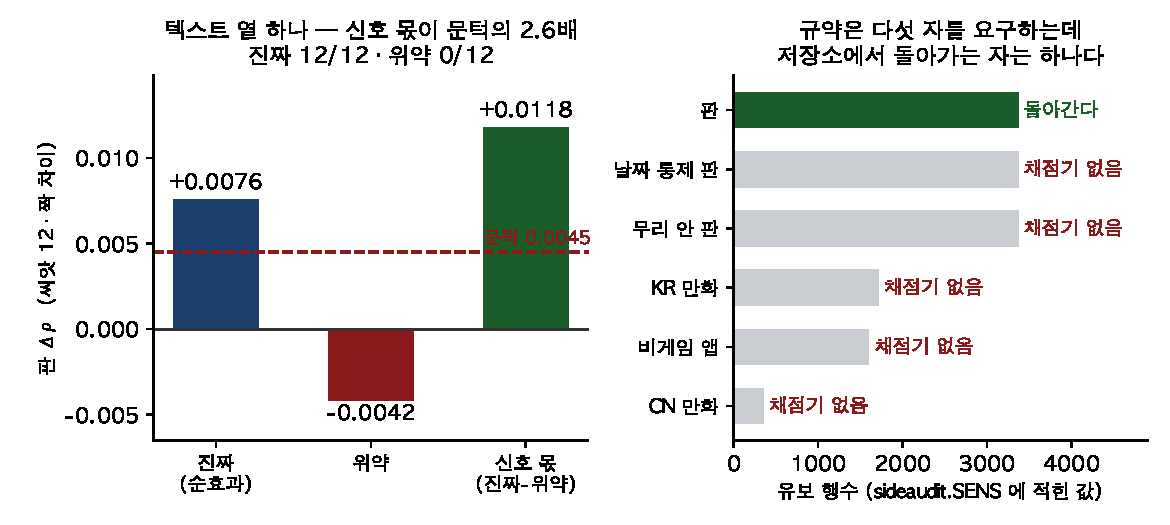
\includegraphics[width=0.99\textwidth]{figs/noruler.pdf}
\caption{왼쪽: 세 팔(씨앗 12 · 짝 차이 · 열 하나). 오른쪽: \texttt{sideaudit.SENS} 에
적힌 자 여섯. \textbf{저장소에서 돌아가는 것은 판 하나다.}}
\end{figure}

\claim{텍스트 열 하나가 챔피언 축 위에 \textbf{문턱의 2.6배}를 더한다. 그리고 그
신호는 \textbf{축이 붙은 여덟 도메인에서 온다} --- 그 몫이 $+0.01206$ 이고 축이 없는
셋은 $-0.00022$ 다. 노트 678 이 경계한 이웃/구조 효과가 아니다.}
{씨앗 40 에서 신호 몫이 $0.0045$ 아래로 내려가면 씨앗 12 의 값은 잡음이었다.
지금 씨앗SE 가 $0.0008$ 이라 신호 몫은 SE 의 15배지만, \textbf{채택 팔은 재적합
팔이라 씨앗 폭이 크다}(노트 609).}

\subsection*{내 예측은 틀렸고, 팔 전에 적은 갱신 예보가 맞았다}

사전등록 예측은 \textbf{③(0 근처)} 였다 --- \emph{``텍스트 신호의 상당 부분이 이미 표
축에 들어 있을 것''}. 근거 셋 중 하나가 \emph{``갈래 어휘가 제목에 있고 \texttt{gen}
이 이미 그것을 나른다''} 였다.

관문 ③ 을 \textbf{팔보다 먼저} 쟀고 그 근거가 무너졌다 --- \texttt{gen} 과의 겹침이
게임 $0.107$ · 만화 $0.011$ · \textbf{애니 $0.007$} 로 \emph{거의 직교}다. 겹치는 것은
\texttt{trend\_*} · \texttt{wiki\_*}(관심도 시계열)이고 최대가 모바일 $0.300$ 이다.
\textbf{제목은 갈래가 아니라 관심도의 대용물이면서 그 위에 증분을 낸다.}

그래서 \textbf{팔이 끝나기 전에} 갱신 예보를 대장에 적고 커밋했다 --- 노트 675 의 용량
곡선을 이 겹침에 적용하면 신호 몫이 양수여야 한다. 그것이 맞았다.

\claim{\textbf{관문을 판정 전에 재면 예보를 두 개 갖게 된다.} 사전등록의 예측과 관문이
가리키는 예측이 갈릴 때, 둘 다 적어 두면 결과가 \emph{어느 근거가 틀렸는지}까지
말해 준다. 여기서는 사전등록이 틀리고 관문이 맞았다.}
{갱신 예보를 결과 뒤에 적으면 그것은 사후 해석이다. 이 논문의 예보는 대장 커밋
시각으로 팔 출력보다 앞선다 --- 그것이 이 주장이 설 수 있는 유일한 근거다.}

\subsection*{그리고 용량 곡선의 도메인 순서는 재현되지 않았다}

노트 675 가 \verb|crowd_share| 에서 겹침 $\leftrightarrow$ 신호 몫 스피어만
$-1.000$ 을 쟀다. 이 축에서는 \textbf{$-0.179$($p{=}0.702$, $n{=}7$)} 로 무늬가 없다.
겹침이 중간인 만화($0.161$)와 게임($0.163$)이 음수인데 더 큰 애니($0.281$)는 양수다.
\textbf{곡선은 판 수준의 부호를 맞혔지만 도메인 순서는 축마다 다르다.} 노트 678 이
\emph{처방으로는 죽었다}를 쟀고 여기에 \emph{진단으로도 축에 딸렸다}가 더해진다.

\section{그런데 확정할 자가 없다}

사전등록 규칙 ①은 \emph{``씨앗 40 과 다섯 자 전부로 확인''} 이었다. 다섯 자를 찾다가
이것을 알았다.

\begin{center}
\begin{tabular}{lll}
\toprule
& 있나 & \\
\midrule
\verb|data/state/manga_kr.json| & \textbf{있다} & KR 만화 명부 1{,}250건 \\
\verb|ingest/app_domain.py| & \textbf{있다} & 앱 \verb|_genre| --- 비게임을 가른다 \\
\verb|sideaudit.SENS| & \textbf{있다} & 자 여섯의 행수와 표본 SD \\
\midrule
그 자들을 계산하는 함수 & \textbf{없다} & \verb|manga_kr| 참조 \verb|.py| 0개 \\
\bottomrule
\end{tabular}
\end{center}

결정적 증거는 채택 커밋이다. 노트 583/586 채택 커밋(\verb|bc0b19860|)의 메시지가
\emph{``판 $0.4663 \to 0.4697$ · KR $0.638 \to 0.684$ · 앱 $0.290 \to 0.505$''} 인데
\textbf{건드린 파일은 \texttt{forms.py} · \texttt{loop.py} · 레코드 · 논문뿐}이다.

\claim{\textbf{그 숫자들은 커밋되지 않은 스크래치 스크립트가 냈다.} 저장소만으로
재현 가능한 자는 \textbf{판 하나}다. 노트 611 이 \emph{``판은 다섯 중 제일 약한
자''}를 쟀으므로 \textbf{판 하나로 채택하는 것은 규약 위반이다.}}
{어딘가에 그 스크립트가 남아 있으면(다른 저장소 · 다른 머신) 이 주장은 ``이
저장소에 없다''로 좁혀진다. 확인한 것은 이 저장소의 전 이력이다.}

\claim{노트 670 이 \emph{``고침이 장부에만 있었다''}를 잡았다. 이것은 같은 층의 다른
자리다 --- \textbf{자가 장부에만 있다.} 그리고 더 나쁘다: 고침은 없으면 결과가
틀리고, \textbf{자는 없으면 결과를 판정할 수 없다.}}
{\texttt{sensitivity()} 가 \texttt{SENS} 를 쓰는 방식이 ``어느 자가 이 효과를 잴 수
있나''를 \emph{조언}하는 것뿐이라면 피해가 작다. 그러나 규약이 그 자들로 채택을
요구하므로 조언에서 끝나지 않는다.}

\section{그래서 무엇을 했나}

\begin{itemize}
\item \verb|sideaudit.SENS| 에 \textbf{경고를 박았다} --- 표를 읽는 다음 사람이 그
      자들을 돌릴 수 있다고 오해하지 않게.
\item \textbf{재건 받아들임 시험 셋을 사전등록했다}: 행 수(1{,}716 · 1{,}600 · 352) ·
      챔피언 기준선($+0.6841$ · $+0.5053$ · $+0.3094$) · 표본 SD. \textbf{셋 다 맞으면}
      기록과 견줄 수 있고 하나라도 어긋나면 \textbf{새 자로 취급한다}(노트 579·580).
\item \textbf{규약 아홉째}: 채택에 쓰는 자는 저장소에서 돌아가야 한다.
\item \textbf{노트 681 의 채택을 보류했다.}
\end{itemize}

예측도 적었다 --- 행 수는 명부와 \verb|_genre| 로 결정론적이니 맞출 수 있지만
\textbf{기준선은 어려울 것}이다. 그때 챔피언 설정과 지금 자료가 다르고, 노트 669 가
방문자 자료 성장으로 사전학습 R$^2$ 가 $0.1639 \to 0.1098$ 이 되는 것을 이미 쟀다.
\textbf{기준선이 어긋나면 그 원인이 채점기가 아니라 자료 성장일 수 있고, 그것을
가르는 것이 재건의 핵심 난점이다.}

\end{document}
